\subsection{C5 MOX Benchmark}
\begin{frame}
\frametitle{Benchmark definition}

\begin{columns}
    \column[t]{4cm}
    \begin{itemize}
        \item 7-group cross-sections: C5G7 \cite{oecdnea_benchmark_2003}.
        \item Capilla et al \cite{capilla_applications_2009}: C5G2.
    \end{itemize}

    \column[t]{6cm}
    \begin{figure}[htbp!]
        \begin{center}
            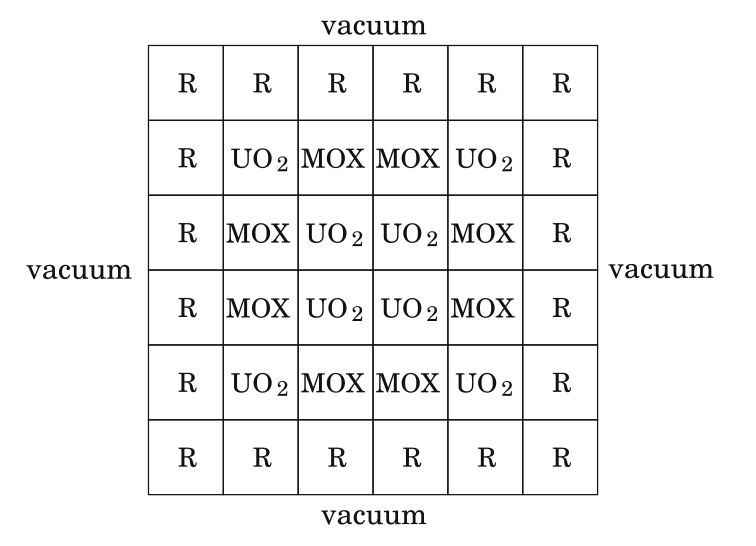
\includegraphics[width=6cm]{figures/bench-config}
        \end{center}
        \caption{2-D C5 MOX benchmark configuration. Image reproduced from \cite{capilla_applications_2009}. $R$ represents the reflectors.}
    \end{figure}
\end{columns}
\end{frame}


\begin{frame}
\frametitle{Benchmark definition (2)}

\begin{columns}
    \column[t]{5.5cm}
    \begin{figure}[htbp!]
        \begin{center}
            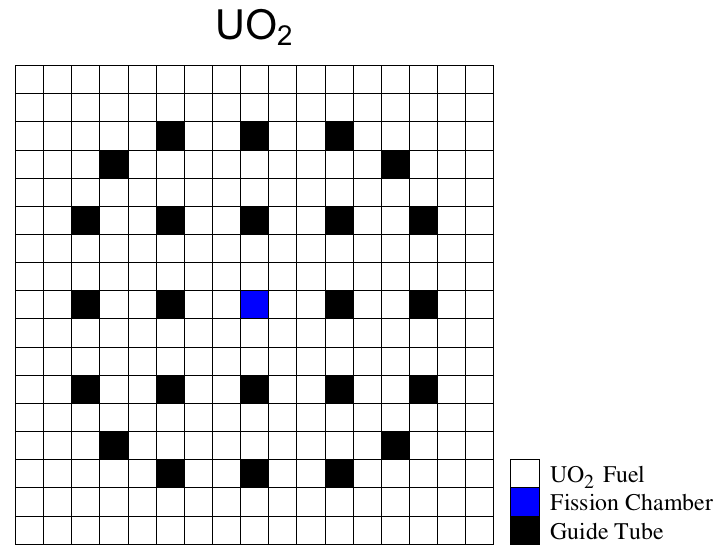
\includegraphics[width=5.5cm]{figures/bench-config2}
        \end{center}
        \caption{UO$_2$ assembly. Image reproduced from \cite{capilla_applications_2009}.}
    \end{figure}

    \column[t]{5.5cm}
    \begin{figure}[htbp!]
        \begin{center}
            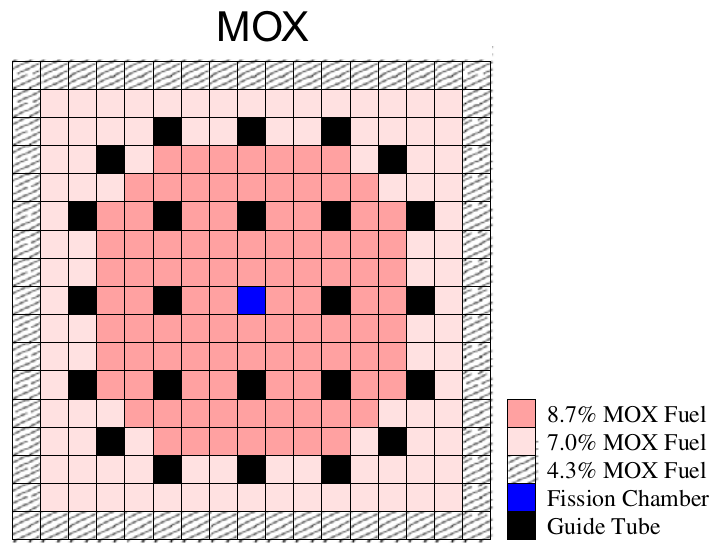
\includegraphics[width=5.5cm]{figures/bench-config3}
        \end{center}
        \caption{MOX assembly. Image reproduced from \cite{capilla_applications_2009}.}
    \end{figure}
\end{columns}
\end{frame}


\begin{frame}
\frametitle{Benchmark geometry}

    \begin{figure}[htbp!]
        \begin{center}
            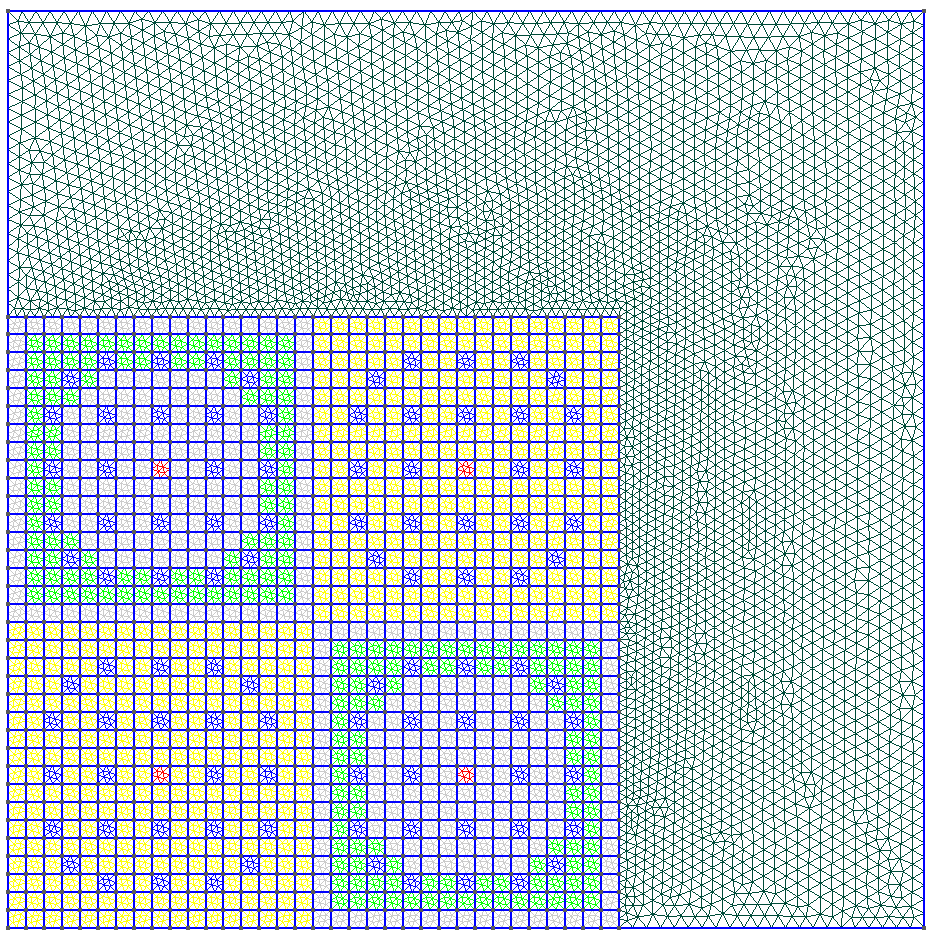
\includegraphics[width=6.cm]{figures/bench-mesh}
        \end{center}
        \caption{Gmsh 2D geometry.}
    \end{figure}

\end{frame}


\subsection{1-D test case}
\begin{frame}
\frametitle{Fixed source}
Comparison between $SP_3$ and Diffusion solutions of the scalar flux.

\begin{columns}

    \column[t]{5cm}
	\begin{figure}[htbp!]
		\begin{center}
			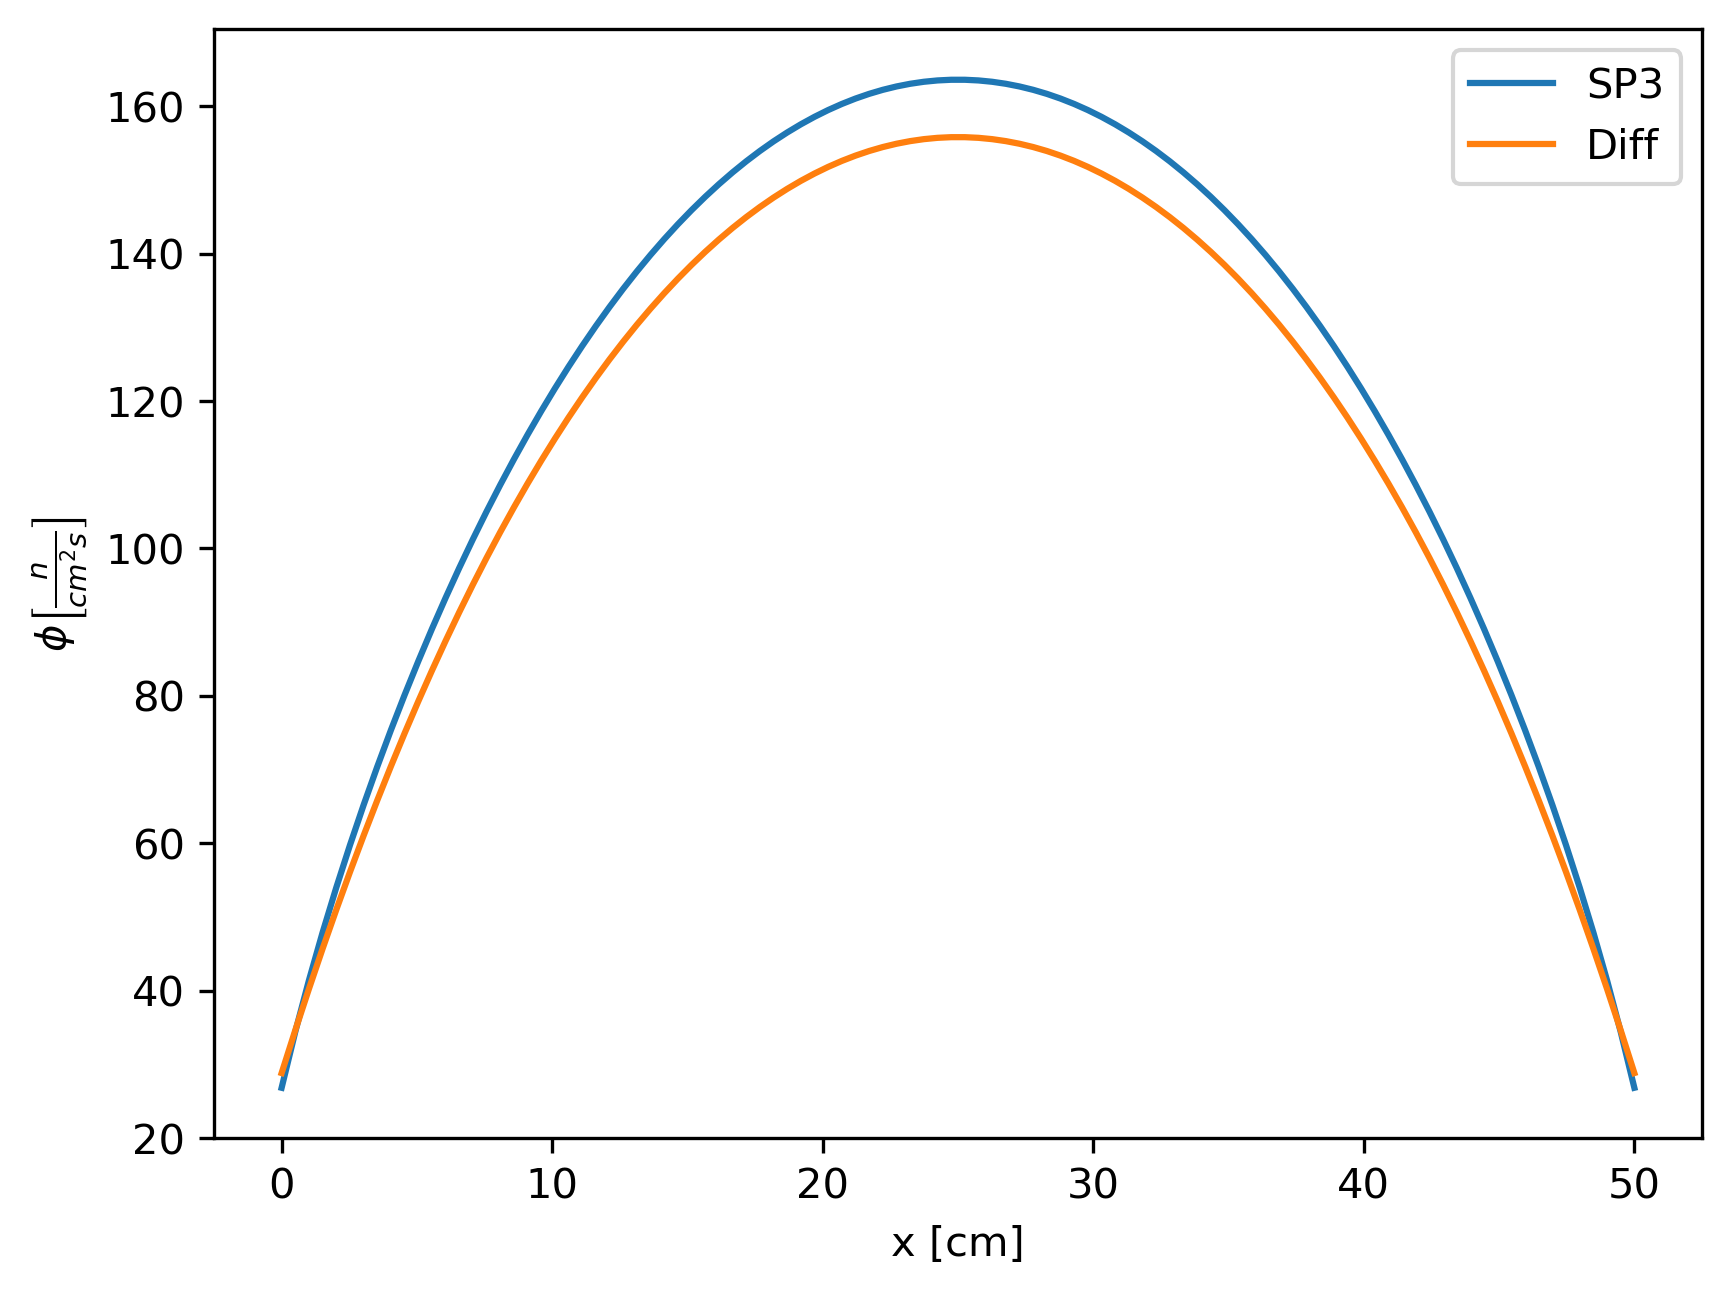
\includegraphics[height=4cm]{figures/output-1g-fixed}
		\end{center}
		\caption{1 group.}
	\end{figure}

	\column[t]{5cm}
	\begin{figure}[htbp!]
		\begin{center}
			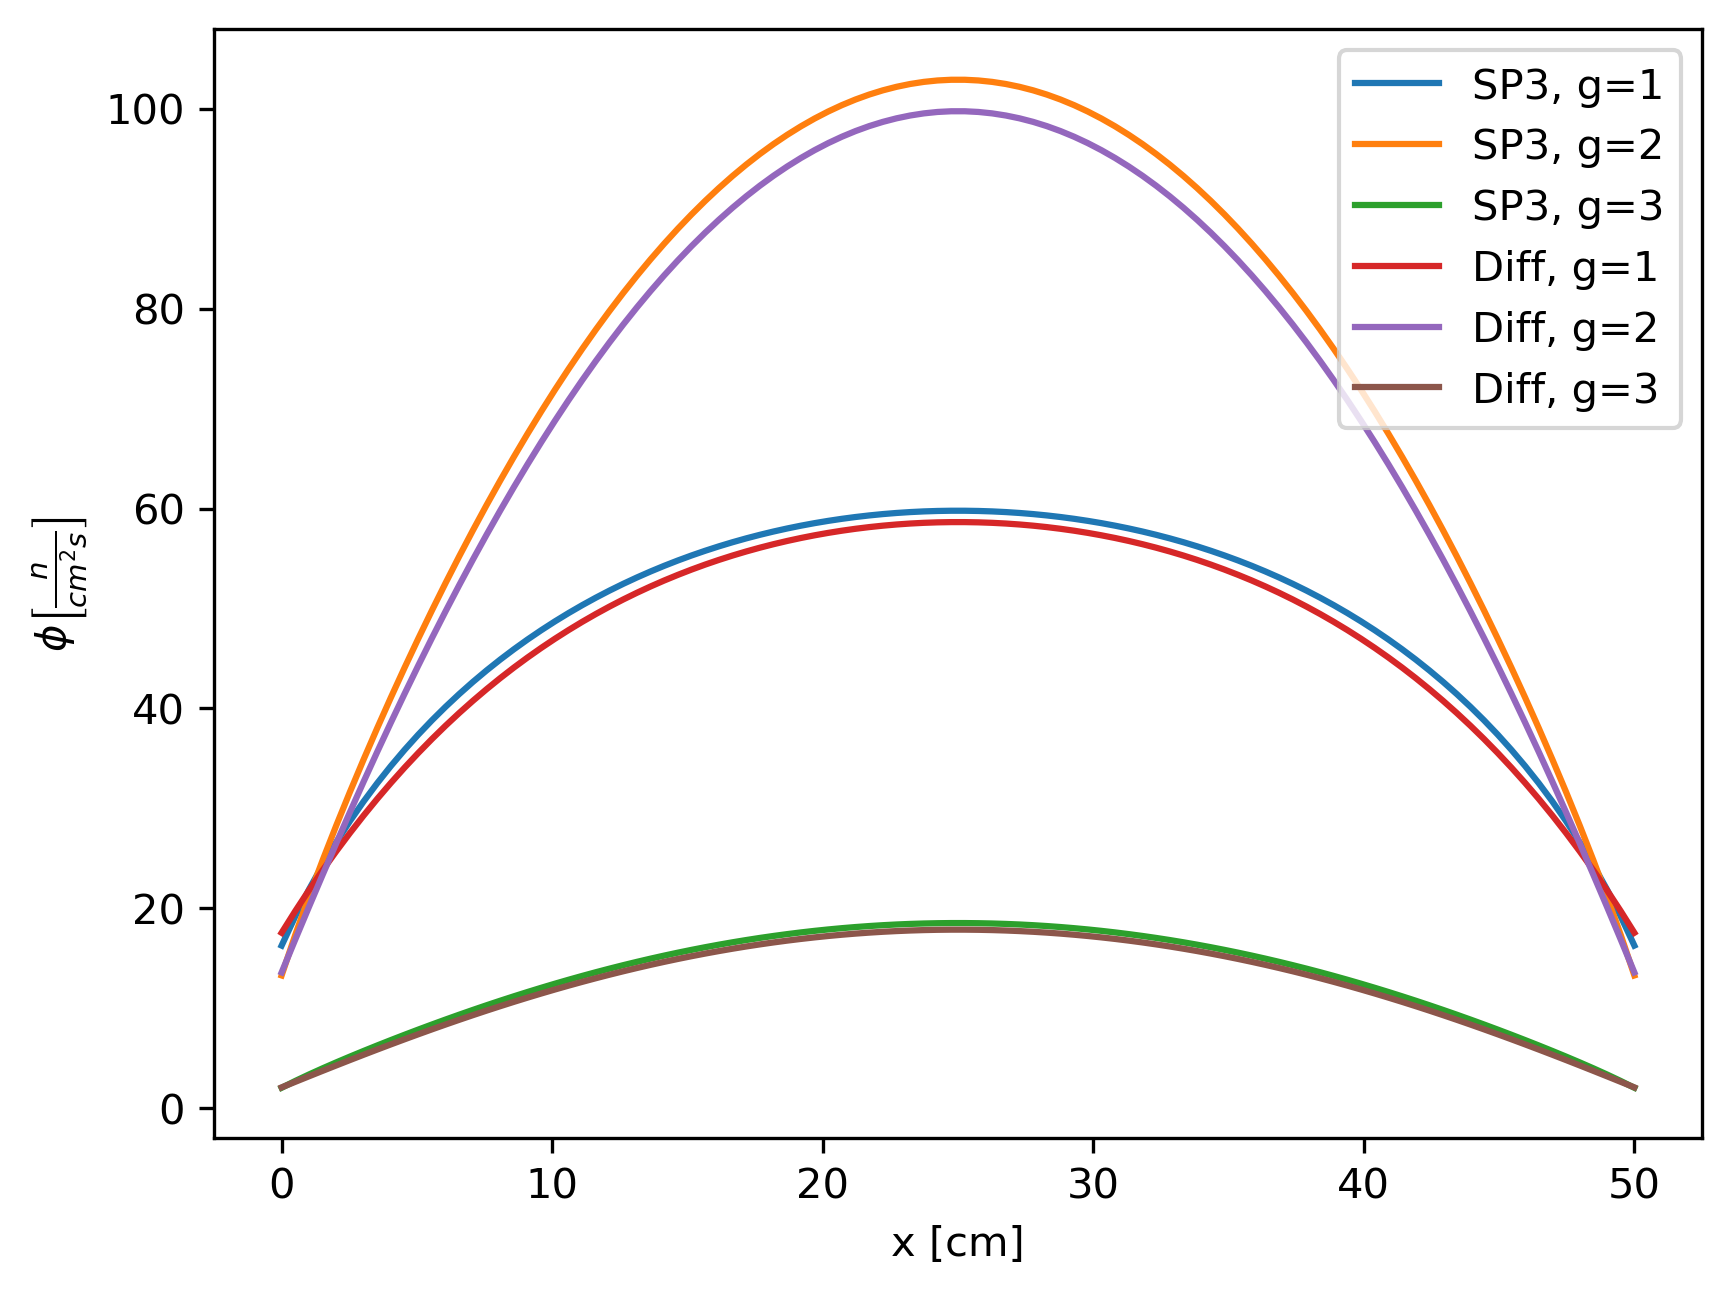
\includegraphics[height=4cm]{figures/output-3g-fixed}
		\end{center}
		\caption{3 groups.}
	\end{figure}
\end{columns}
\end{frame}


\begin{frame}
\frametitle{Eigenvalue problem}

Comparison between $SP_3$ and Diffusion solutions of the scalar flux.
Solutions are normalized to the maximum value of the flux (fast flux for the 3 group case).

\begin{columns}
    \column[t]{5cm}
	\begin{figure}[htbp!]
		\begin{center}
			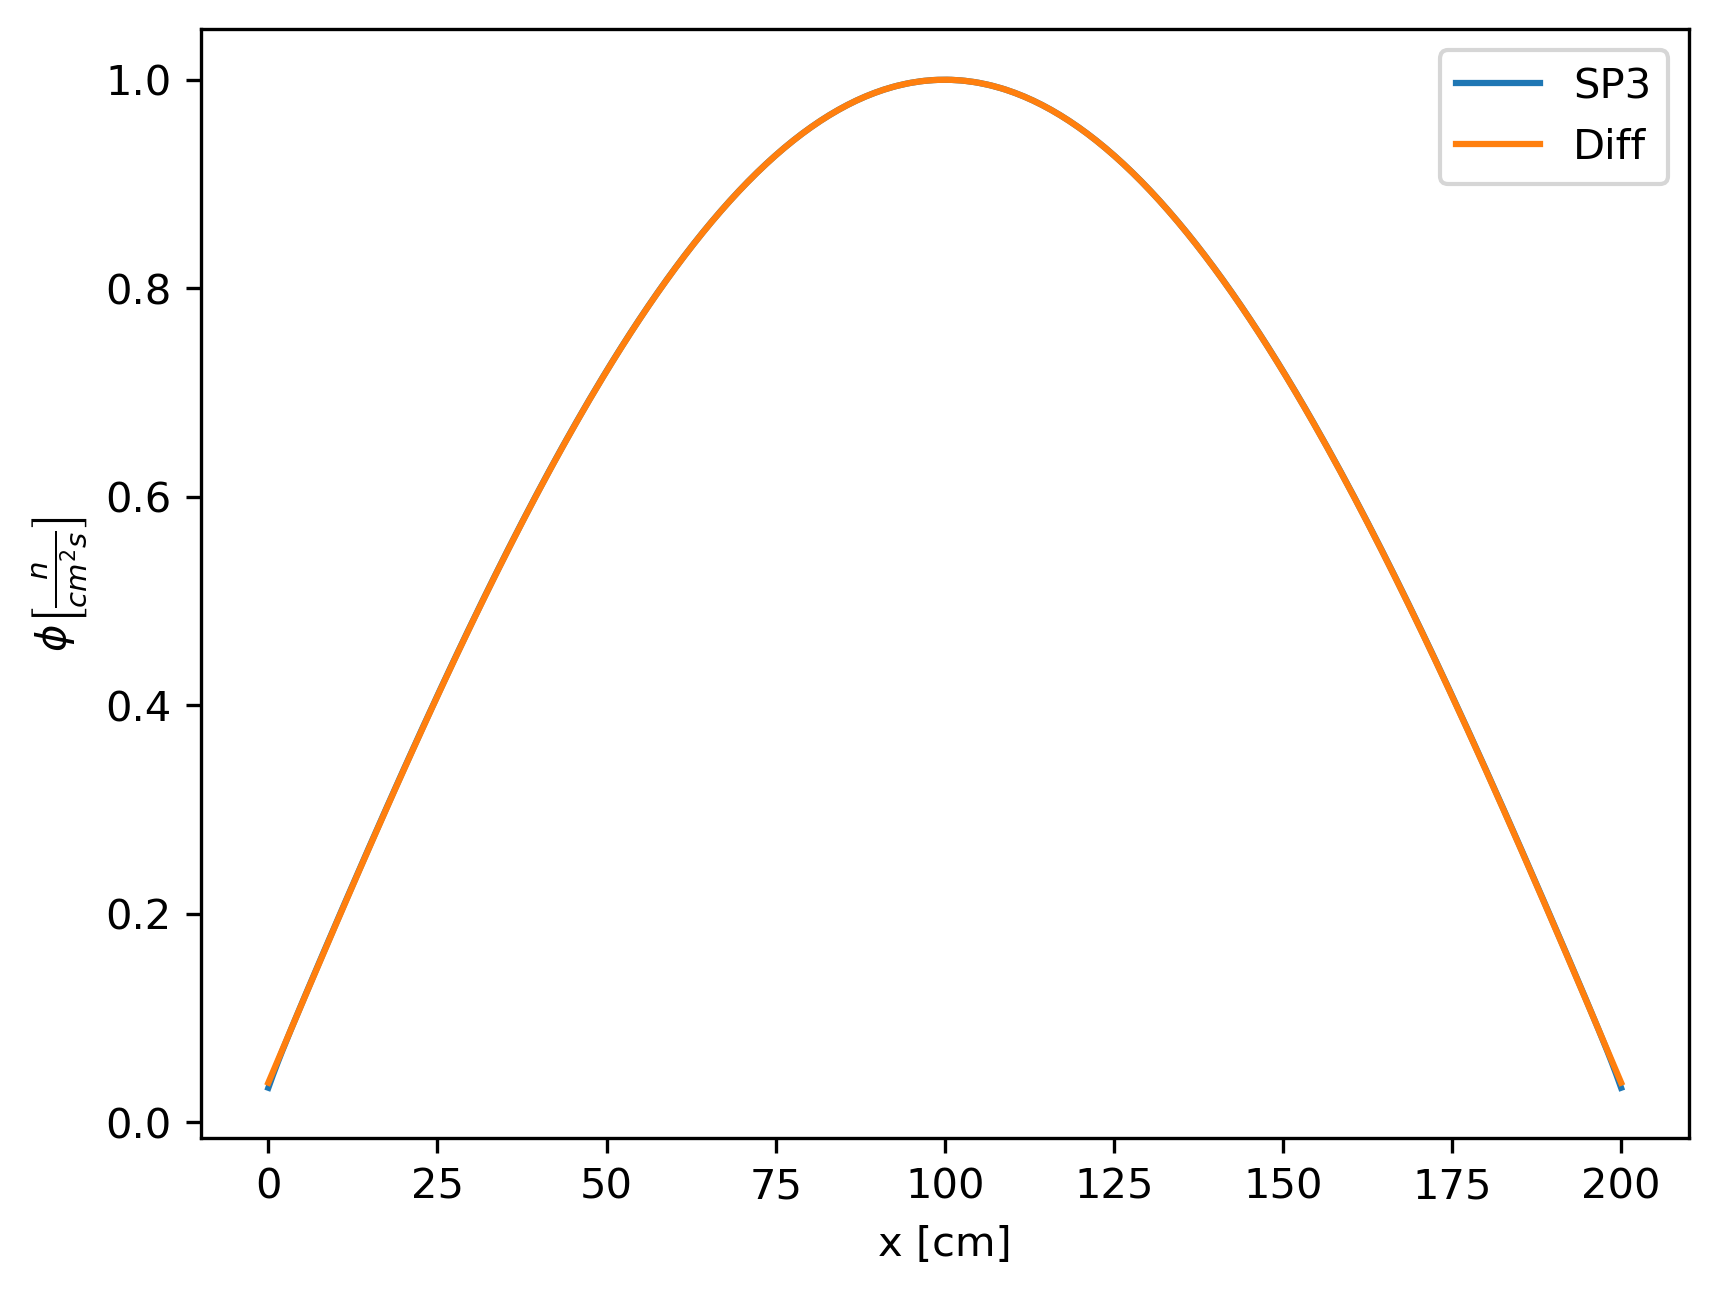
\includegraphics[height=4cm]{figures/output-1g-crit}
		\end{center}
		\caption{1 group.}
	\end{figure}

	\column[t]{5cm}
	\begin{figure}[htbp!]
		\begin{center}
			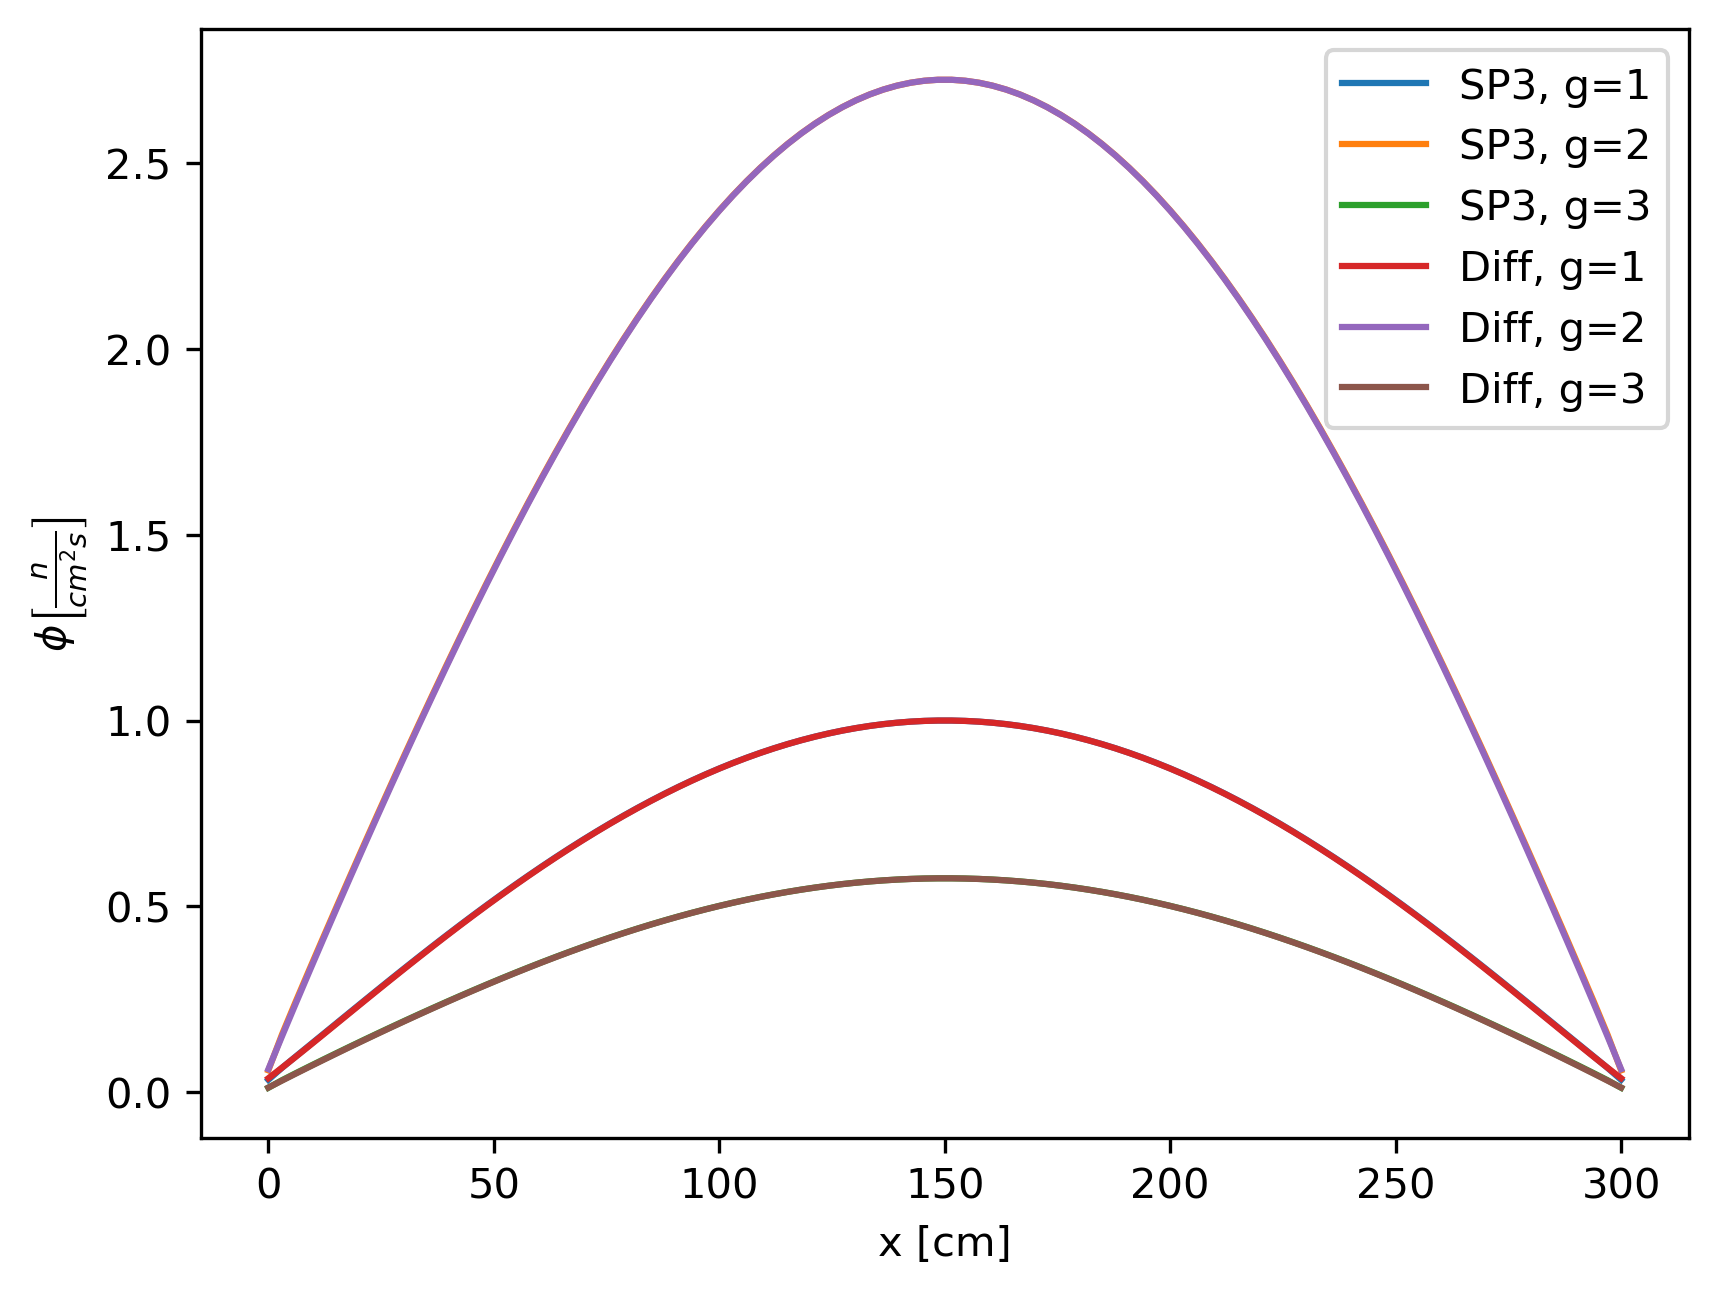
\includegraphics[height=4cm]{figures/output-3g-crit}
		\end{center}
		\caption{3 groups.}
	\end{figure}
\end{columns}
\end{frame}


\subsection{2-D test case}
\begin{frame}
\frametitle{C5G2 MOX Benchmark}
	\begin{table}[htbp!]
	\centering
	\begin{tabular}{lccc}
	\toprule
	 & C5G2 Benchmark      & \multicolumn{2}{c}{SP3}          \\
	\midrule
	Case & $k_{Ref}$       & $k_{SP_3}$ & $\Delta_\rho$ [pcm] \\
	\midrule
	Heterogeneous & 0.96969  & 0.97106  & 145  \\
	Homogeneous   & 0.96983  & 0.97061  &  83  \\
	\bottomrule
	\end{tabular}
	\label{tab:2d-keff}
	\end{table}
\end{frame}

\begin{frame}
\frametitle{C5G2 MOX Benchmark (2)}
	\begin{figure}[htbp!]
		\begin{center}
			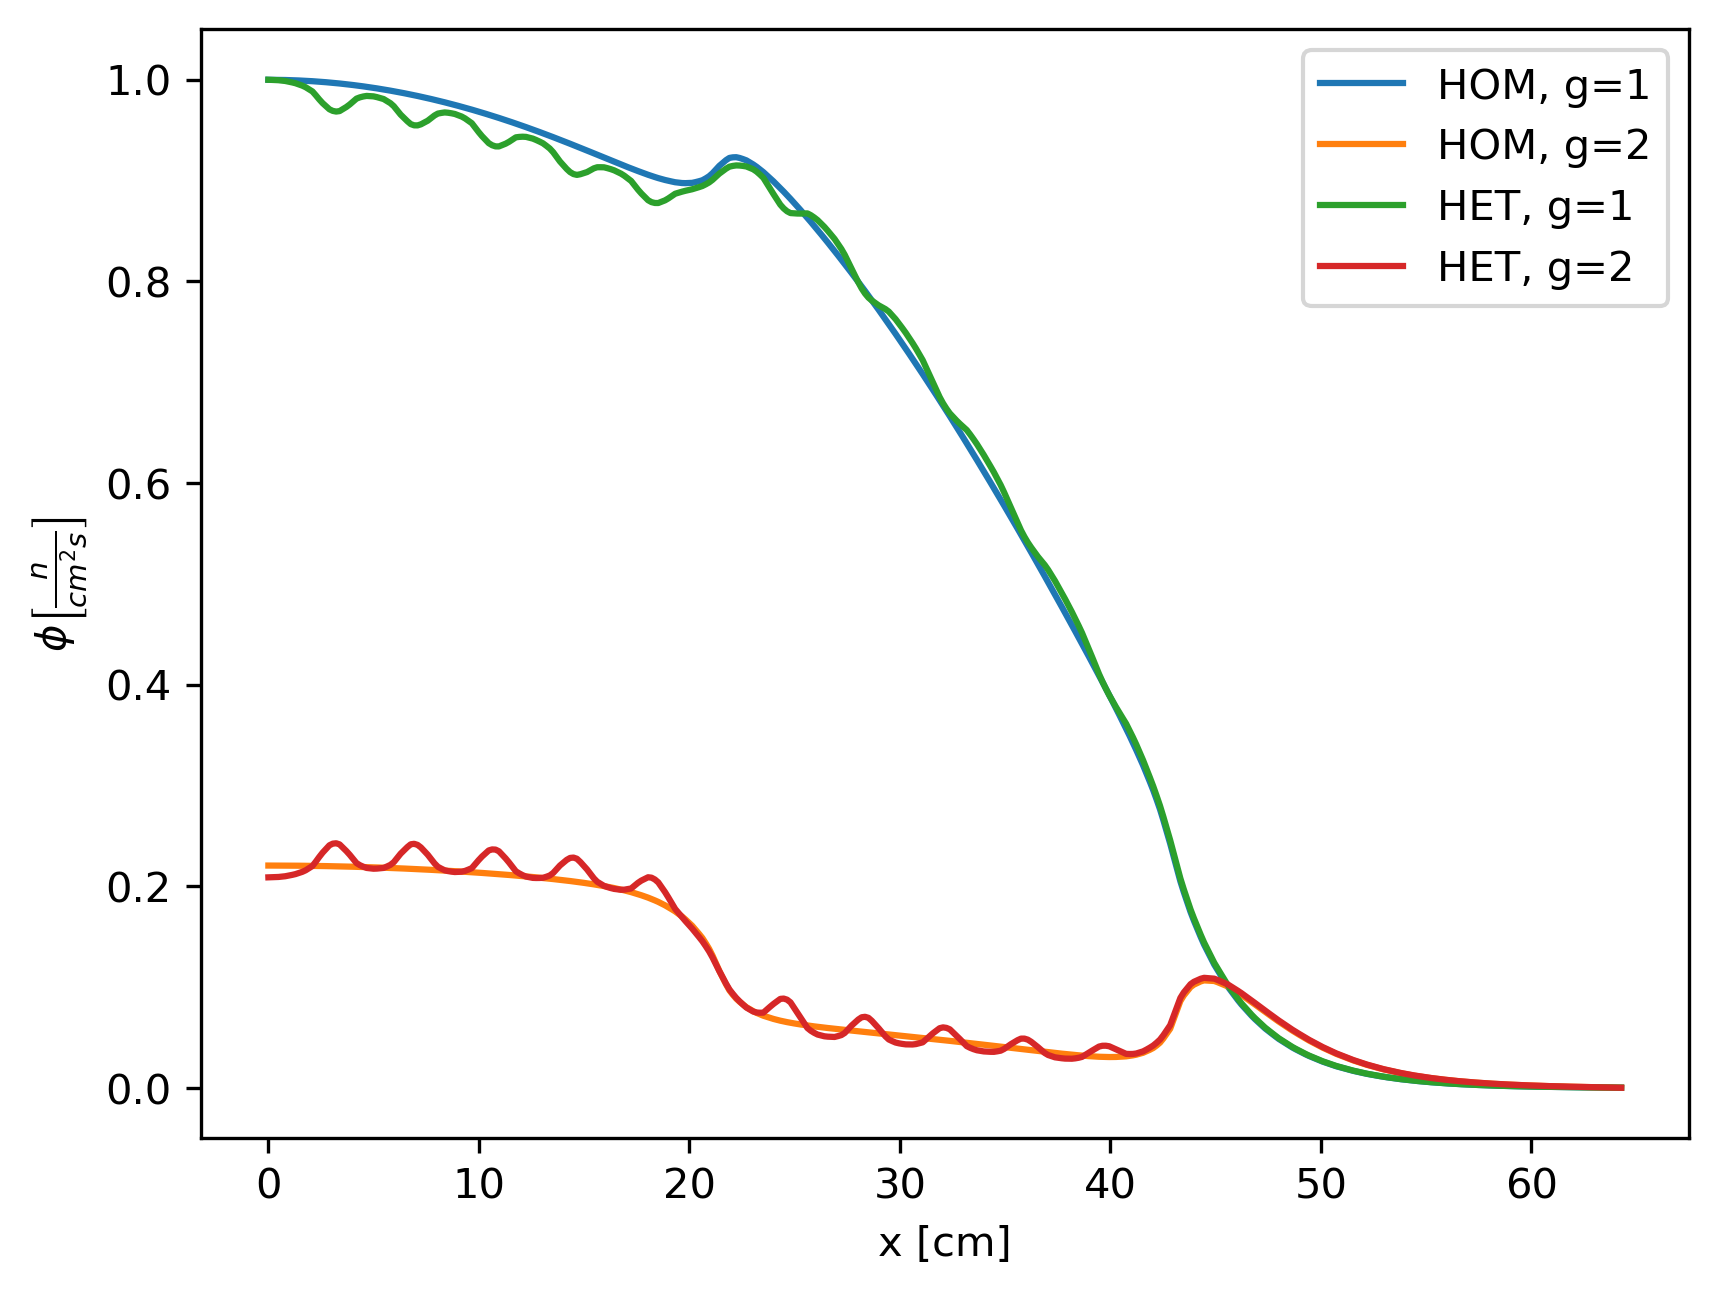
\includegraphics[height=5cm]{{figures/output-2g}}
		\end{center}
		\caption{Comparison of the heterogenous and homogeneous cases scalar flux.}
	\end{figure}
\end{frame}

\begin{frame}
\begin{columns}
\frametitle{C5G2 MOX Benchmark (3)}

    \column[t]{5cm}
	\begin{figure}[htbp!]
		\begin{center}
			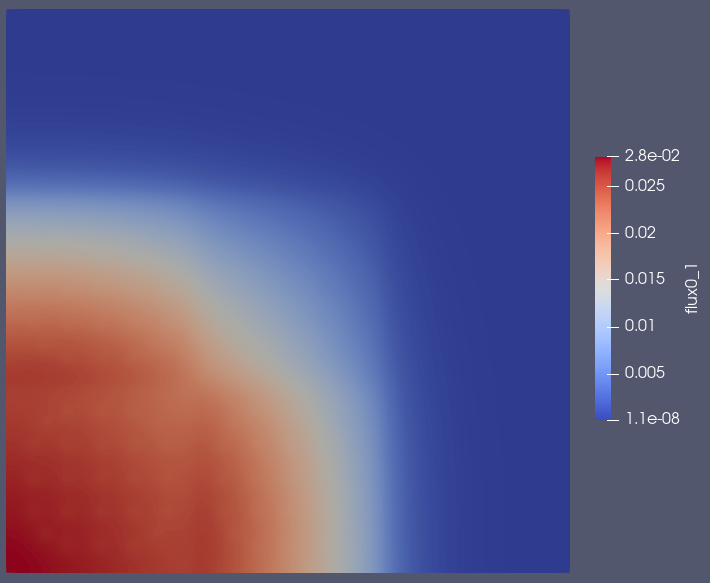
\includegraphics[height=4cm]{figures/flux0_1}
		\end{center}
		\caption{$\Phi_{0, 1}$.}
	\end{figure}

	\column[t]{5cm}
	\begin{figure}[htbp!]
		\begin{center}
			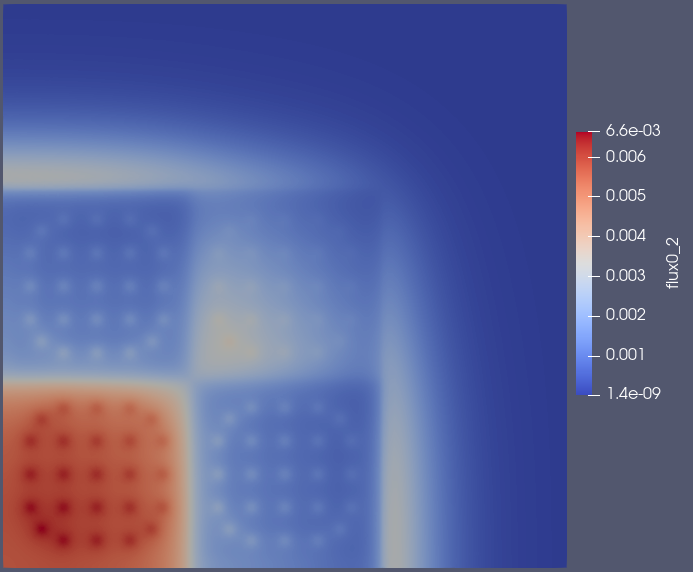
\includegraphics[height=4cm]{figures/flux0_2}
		\end{center}
		\caption{$\Phi_{0, 2}$.}
	\end{figure}
\end{columns}
\end{frame}

\begin{frame}
\frametitle{C5G2 MOX Benchmark (4)}
\begin{columns}
    \column[t]{5cm}
	\begin{figure}[htbp!]
		\begin{center}
			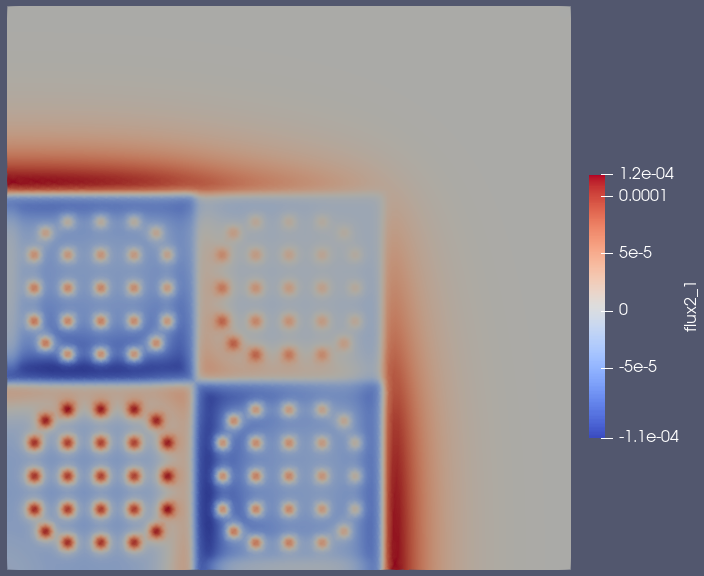
\includegraphics[height=4cm]{figures/flux2_1}
		\end{center}
		\caption{$\Phi_{2, 1}$.}
	\end{figure}

	\column[t]{5cm}
	\begin{figure}[htbp!]
		\begin{center}
			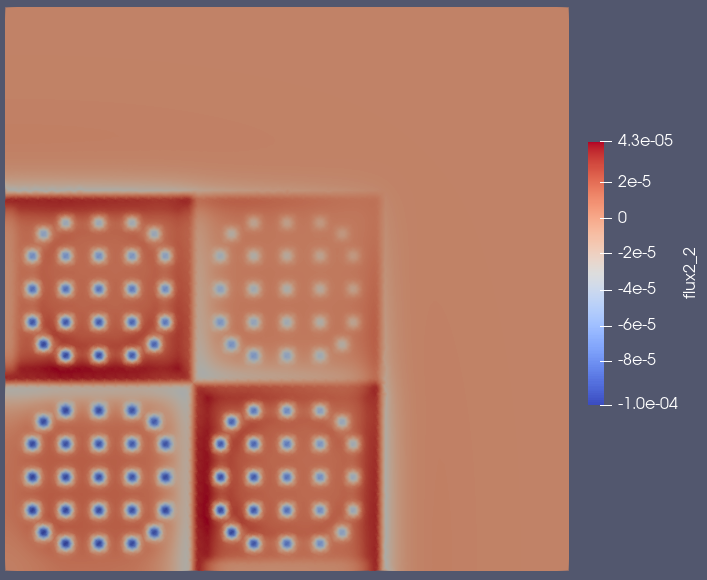
\includegraphics[height=4cm]{figures/flux2_2}
		\end{center}
		\caption{$\Phi_{2, 2}$.}
	\end{figure}
\end{columns}
\end{frame}